\documentclass[11pt]{article}
\usepackage{graphicx}
\usepackage[bookmarks=true]{hyperref}
\usepackage{bookmark}
\usepackage{hyperref}
\usepackage{float}
\usepackage{wrapfig}

\usepackage{array}
\newcolumntype{L}[1]{>{\raggedright\let\newline\\\arraybackslash\hspace{0pt}}m{#1}}
\newcolumntype{C}[1]{>{\centering\let\newline\\\arraybackslash\hspace{0pt}}m{#1}}
\newcolumntype{R}[1]{>{\raggedleft\let\newline\\\arraybackslash\hspace{0pt}}m{#1}}

\begin{document}

\begin{titlepage}
\begin{flushright}


\includegraphics[width=380px]{./images/University_of_Pretoria_Logo.png}
\newline
\newline

\textbf {\LARGE Software Requirements Specification} \newline

\textbf {\Large Linphone for Andriod Group Chat (Waterfall)}\newline

\textbf {\large Version: 2.0}\newline

\centering \textbf {\large Authors:}

\begin{table}[H]
\large
\centering
\begin{tabular}{rl}
	Izak Blom & 13126777 \\
	David Breetzke & 12056503 \\
	Paul Engelke & 13093500 \\
	Prenolan Govender & 13102380 \\
	Jessica Lessev & 13049136 \\
\end{tabular}
\end{table}

Date: 26 May 2015

\end{flushright}
\end{titlepage}

\setcounter{tocdepth}{3}
\tableofcontents

\newpage
\section{Revision History}
\begin{table}[h]
\begin{tabular}{llll}
\textbf{Date}          & \textbf{Description}  & \textbf{Author}       & \textbf{Comments}   \\ \hline
\multicolumn{1}{|R{2.5cm}|}{26/05/2015} & \multicolumn{1}{L{5.5cm}|}{Document Creation} & \multicolumn{1}{l|}{Team Eclectic} & \multicolumn{1}{L{4cm}|}{Version 1} \\ \hline
\multicolumn{1}{|l|}{} & \multicolumn{1}{l|}{} & \multicolumn{1}{l|}{} & \multicolumn{1}{l|}{} \\ \hline
\multicolumn{1}{|l|}{} & \multicolumn{1}{l|}{} & \multicolumn{1}{l|}{} & \multicolumn{1}{l|}{} \\ \hline
\multicolumn{1}{|l|}{} & \multicolumn{1}{l|}{} & \multicolumn{1}{l|}{} & \multicolumn{1}{l|}{} \\ \hline
\multicolumn{1}{|l|}{} & \multicolumn{1}{l|}{} & \multicolumn{1}{l|}{} & \multicolumn{1}{l|}{} \\ \hline
\multicolumn{1}{|l|}{} & \multicolumn{1}{l|}{} & \multicolumn{1}{l|}{} & \multicolumn{1}{l|}{} \\ \hline
\multicolumn{1}{|l|}{} & \multicolumn{1}{l|}{} & \multicolumn{1}{l|}{} & \multicolumn{1}{l|}{} \\ \hline
\multicolumn{1}{|l|}{} & \multicolumn{1}{l|}{} & \multicolumn{1}{l|}{} & \multicolumn{1}{l|}{} \\ \hline
\multicolumn{1}{|l|}{} & \multicolumn{1}{l|}{} & \multicolumn{1}{l|}{} & \multicolumn{1}{l|}{} \\ \hline
\multicolumn{1}{|l|}{} & \multicolumn{1}{l|}{} & \multicolumn{1}{l|}{} & \multicolumn{1}{l|}{} \\ \hline
\end{tabular}
\end{table}

\section{Document Approval}
\begin{table}[h]
\begin{tabular}{llll}
\textbf{Signature}     & \textbf{Printed Name} & \textbf{Title}        & \textbf{Comments}     \\ \hline
\multicolumn{1}{|l|}{} & \multicolumn{1}{L{4.5cm}|}{} & \multicolumn{1}{L{4cm}|}{} & \multicolumn{1}{L{4cm}|}{} \\ \hline
\multicolumn{1}{|l|}{} & \multicolumn{1}{l|}{} & \multicolumn{1}{l|}{} & \multicolumn{1}{l|}{} \\ \hline
\multicolumn{1}{|l|}{} & \multicolumn{1}{l|}{} & \multicolumn{1}{l|}{} & \multicolumn{1}{l|}{} \\ \hline
\multicolumn{1}{|l|}{} & \multicolumn{1}{l|}{} & \multicolumn{1}{l|}{} & \multicolumn{1}{l|}{} \\ \hline
\multicolumn{1}{|l|}{} & \multicolumn{1}{l|}{} & \multicolumn{1}{l|}{} & \multicolumn{1}{l|}{} \\ \hline
\multicolumn{1}{|l|}{} & \multicolumn{1}{l|}{} & \multicolumn{1}{l|}{} & \multicolumn{1}{l|}{} \\ \hline
\multicolumn{1}{|l|}{} & \multicolumn{1}{l|}{} & \multicolumn{1}{l|}{} & \multicolumn{1}{l|}{} \\ \hline
\multicolumn{1}{|l|}{} & \multicolumn{1}{l|}{} & \multicolumn{1}{l|}{} & \multicolumn{1}{l|}{} \\ \hline
\multicolumn{1}{|l|}{} & \multicolumn{1}{l|}{} & \multicolumn{1}{l|}{} & \multicolumn{1}{l|}{} \\ \hline
\multicolumn{1}{|l|}{} & \multicolumn{1}{l|}{} & \multicolumn{1}{l|}{} & \multicolumn{1}{l|}{} \\ \hline
\end{tabular}
\end{table}

\newpage
\section{Introduction}
\subsection{Purpose}
\subsection{Scope}
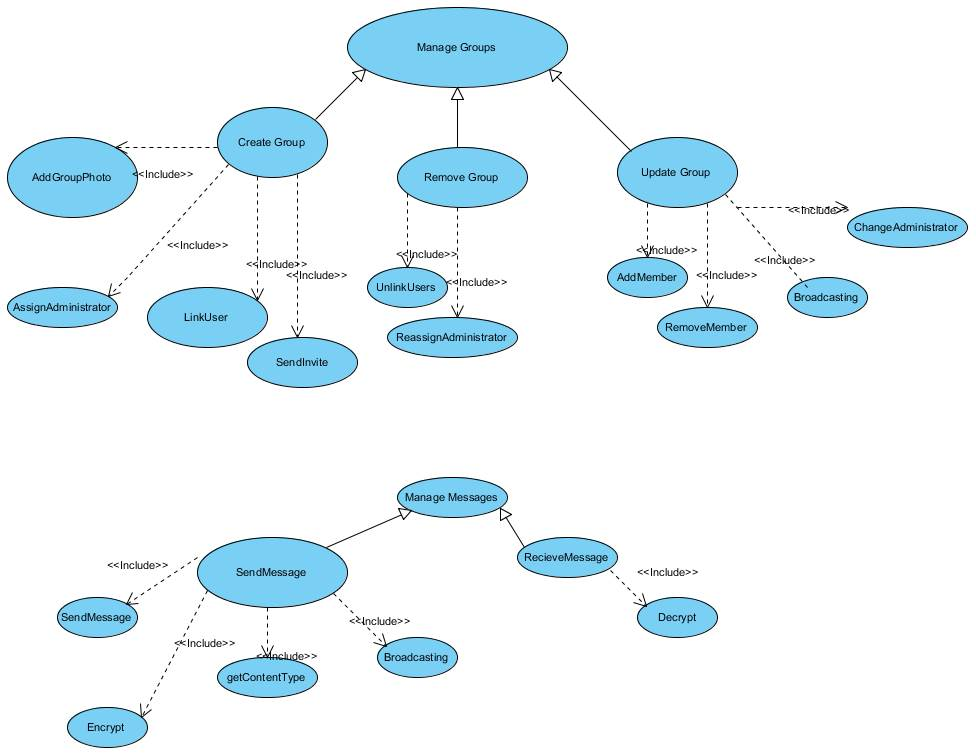
\includegraphics[width=380px]{./images/scope.png}
\subsection{Definitions, Acronyms \& Abbreviations}
%\subsection{References}
\subsection{Overview}

\section{Specific Requirements}
%\subsection{External Interface Requirements}
%\subsubsection{User Interfaces}
%\subsubsection{Hardware Interfaces}
%\subsubsection{Software Interfaces}
%\subsubsection{Communication Interfaces}

\subsection{Functional Requirements}
\subsubsection{Group Chat Creation (critical)}
The ManageGroups module provides services to create, update and remove or leave groups\newline
\newline
\bullet ManageGroups.CreateGroup – Priority: Critical.\newline
\bullet	This use case allows users to create a group where more than 1 contact can communicate simultaneously together.\newline
\bullet	This creates a space where messages can be exchanged between users that are members of the groups \newline
\newline
	Services Contract: \newline
	\newline
\bullet The CreateGroupRequest identifies the user that is creating the group and automatically assigns this user to be the administrator.\newline
\bullet It allows the user to select contacts that the user wishes to add to the group.\newline
\bullet The group members are then notified by receiving an invitation to join and are linked to the group.\newline
\bullet The service has three pre-conditions and three post-conditions\newline
\newline Pre-conditions\newline
For each of the pre-conditions below an exception is introduced which is raised by the service to notify the caller that the service is not being provided as the pre-condition associated with that exception has not been met.\newline
The group will not be created if one of the following scenarios occurs:\newline
\newline
\bullet	User must have Linphone Service\newline
\bullet	No other group with the same name may exist \newline
\bullet	The user may not create the group unless there is at least one member/contact added.\newline
\newline
Post-Conditions\newline
The post-conditions specify the conditions which must hold true when the service has been provided.\newline
\newline
\bullet	User is automatically assigned administrator rights\newline
\bullet	An invite is sent to users to ask them if they want to be part of the group\newline
\bullet	The group is created with the respective profiles and members \newline
\newline
\includegraphics[width=380px]{./images/serviceContract-createGroup.png}
\newline
Functional Requirements\newline
 The functional requirements specify what the system should do and how the system should behave. Each use case has functional requirements and these specify the functions required by the use cases in order to use the service specified in the services contract. Each functional requirement is either checking for a post-condition or a precondition or both.\newline
 \newline
\includegraphics[width=380px]{./images/functionalReq-createGroup.png}
 \newline
Process Specification \newline
 \newline
 \includegraphics[width=380px]{./images/process-createGroup.png}
  \newline
 First the user creating the group fills in the relative details such as the group name and adds members to the group. Each of these members needs to have the Linphone service to be added to the group. If the contacts do not have Linphone, an error is thrown. Next the user tries to create the group. If less than 1 member is added then an error is thrown and the group is not created. If more than one member was added then the system continues to check whether there are any other groups with the same name. If so, then an exception is thrown, otherwise the user is assigned as group administrator, an invite is sent to the members and the group is created.
 \newline
\subsubsection{Group Chat Deletion (critical)}
\subsubsection{Group Chat Updating (critical)}
\subsubsection{Adding Members (critical)}
\subsubsection{Removing Members (critical)}
\subsubsection{Sending Messages (critical)}
\subsubsection{Sending Voice Recordings (Important)}
%\subsection{Non-Functional Requirements}

%\section{Requirements Traceability Matrix}

\end{document}